% "Your VLA is Secretly kNN" -- A1 portrait workshop poster, three sections (left / middle / right).
% Build: `make` in this directory (collects results, renders figures + numbers.tex, runs lualatex).
\documentclass{article}
\usepackage[paperwidth=594mm,paperheight=841mm,margin=0mm]{geometry}
\usepackage{fontspec}
\usepackage{unicode-math}
\setmainfont{Inter}[Numbers=Proportional]
\newfontfamily\display{Inter Display}
\setmathfont{FiraMath-Regular.otf}
\usepackage{xcolor,graphicx,booktabs,tabularx,array,enumitem,colortbl}
\usepackage{tikz}
\usetikzlibrary{arrows.meta,decorations.markings,calc,positioning,shapes.geometric}
\usepackage[poster,skins,fitting]{tcolorbox}

% ---- colour roles (validated with the dataviz palette checker) -------------------------------------------
\definecolor{page}{HTML}{EDEFF2}
\definecolor{panel}{HTML}{FFFFFF}
\definecolor{ink}{HTML}{0B0B0B}
\definecolor{ink2}{HTML}{4A4946}
\definecolor{muted}{HTML}{898781}
\definecolor{hair}{HTML}{DCDEE2}
\definecolor{tint}{HTML}{F5F6F8}
\definecolor{titlebg}{HTML}{121821}
\definecolor{knn}{HTML}{EB6834}      % kNN / retrieval (ours)
\definecolor{learned}{HTML}{2A78D6}  % learned models (DiT, VLA)
\definecolor{human}{HTML}{9A988F}    % human demonstrations, generic encoders
\definecolor{ladderA}{HTML}{86B6EF}  % generic VLM
\definecolor{ladderB}{HTML}{2A78D6}  % robot-pretrained VLA
\definecolor{ladderC}{HTML}{104281}  % LIBERO fine-tuned VLA

% generated by scripts/make_figures.py -- do not edit
\newif\ifhavewins
\havewinstrue
\newif\ifhavepi
\havepitrue
\newif\ifhavediag
\havediagtrue
\newif\ifhavekeys
\havekeystrue
\newif\ifhaveneighbors
\haveneighborstrue
\newif\ifhaveplus
\haveplustrue
\newcommand{\KnnAvg}{91.7}
\newcommand{\KnnSpatial}{88.0}
\newcommand{\KnnObject}{99.8}
\newcommand{\KnnGoal}{97.6}
\newcommand{\KnnLong}{81.4}
\newcommand{\KnnEpisodes}{2,000}
\newcommand{\DitDocsAvg}{90.6}
\newcommand{\PiFiveAvg}{97.5}
\newcommand{\OpenVlaAvg}{76.5}
\newcommand{\AblBase}{90.6}
\newcommand{\AblNoLang}{63.0}
\newcommand{\AblNoLangGoal}{8}
\newcommand{\AblPixels}{57.3}
\newcommand{\AblKOne}{79.8}
\newcommand{\AblDino}{83.0}
\newcommand{\AblOpenLoop}{92.5}
\newcommand{\DemosTen}{77.8}
\newcommand{\DitOurs}{68.8}
\newcommand{\DitTrainMed}{0.0016}
\newcommand{\HumanMed}{0.0018}
\newcommand{\DitKnnMed}{0.0109}
\newcommand{\KnnSpreadMed}{0.0095}
\newcommand{\GripAgree}{83}
\newcommand{\DitChunks}{789}
\newcommand{\DiagN}{30}
\newcommand{\DiagOkMax}{3.9}
\newcommand{\DiagBadMin}{6.0}
\newcommand{\DiagBad}{4}
\newcommand{\DitSpatial}{87.0}
\newcommand{\DitObject}{98.2}
\newcommand{\DitGoal}{93.8}
\newcommand{\DitLong}{83.2}
\newcommand{\PiFiveSpatial}{97.0}
\newcommand{\PiFiveObject}{99.0}
\newcommand{\PiFiveGoal}{98.0}
\newcommand{\PiFiveLong}{96.0}
\newcommand{\KnnSeedTwo}{92.4}
\newcommand{\KnnHiRes}{91.5}
\newcommand{\KnnSmolLibero}{77.8}
\newcommand{\KnnSmolBase}{62.3}
\newcommand{\KnnSmolLiberoGrid}{85.3}
\newcommand{\KnnSmolBaseGrid}{74.5}
\newcommand{\KnnPlainResnet}{87.3}
\newcommand{\KnnPlainResnetMean}{70.3}
\newcommand{\KnnPlainDino}{74.5}
\newcommand{\KnnPiLibero}{71.0}
\newcommand{\KnnPiBase}{\pending}
\newcommand{\KnnPiLiberoAvOne}{72.0}
\newcommand{\VlaSmol}{80.0}
\newcommand{\VlaPi}{97.0}
\newcommand{\SwapSmol}{107}
\newcommand{\SwapSmolMean}{97}
\newcommand{\SwapPi}{73}
\newcommand{\SwapPiMean}{\pending}
\newcommand{\HeadSmolOwn}{0.79}
\newcommand{\HeadSmolOwnOne}{0.65}
\newcommand{\HeadSmolBefore}{0.65}
\newcommand{\HeadSmolBeforeOne}{0.38}
\newcommand{\HeadSmolResnet}{0.66}
\newcommand{\HeadSmolResnetOne}{0.44}
\newcommand{\HeadSmolSelf}{0.99}
\newcommand{\HeadSmolNnVla}{0.0016}
\newcommand{\HeadSmolNnDemo}{0.0020}
\newcommand{\HeadPiOwn}{0.88}
\newcommand{\HeadPiOwnOne}{0.81}
\newcommand{\HeadPiBefore}{\pending}
\newcommand{\HeadPiBeforeOne}{\pending}
\newcommand{\HeadPiResnet}{0.90}
\newcommand{\HeadPiResnetOne}{0.78}
\newcommand{\HeadPiSelf}{0.99}
\newcommand{\HeadPiNnVla}{0.0012}
\newcommand{\HeadPiNnDemo}{0.0020}
\newcommand{\VlaPiSpatial}{96.0}
\newcommand{\KnnPiLiberoSpatial}{73.0}
\newcommand{\VlaPiObject}{99.0}
\newcommand{\KnnPiLiberoObject}{72.0}
\newcommand{\VlaPiGoal}{96.0}
\newcommand{\KnnPiLiberoGoal}{80.0}
\newcommand{\VlaPiLong}{97.0}
\newcommand{\KnnPiLiberoLong}{59.0}
\newcommand{\KnnPiLiberoZ}{79.3}
\newcommand{\KnnPiBaseZ}{81.3}
\newcommand{\KnnPiLiberoLf}{79.0}
\newcommand{\KnnPiBaseLf}{82.3}
\newcommand{\KnnPiLiberoLt}{84.5}
\newcommand{\KnnPiBaseLt}{88.5}
\newcommand{\BestLookupPi}{84.5}
\newcommand{\BestLookupSmol}{85.3}
\newcommand{\VlaSmolSpatial}{76.0}
\newcommand{\VlaSmolObject}{90.0}
\newcommand{\VlaSmolGoal}{88.0}
\newcommand{\VlaSmolLong}{66.0}
\newcommand{\KnnPiBaseMulti}{84.5}
\newcommand{\KnnPiLiberoMulti}{80.5}
\newcommand{\KnnPiBasePca}{88.0}
\newcommand{\KnnPiLiberoPca}{79.8}
\newcommand{\KnnLearnt}{90.5}
\newcommand{\KnnFullLearnt}{91.5}
\newcommand{\NmFairRho}{0.90}
\newcommand{\NmFairGlobalRho}{0.31}
\newcommand{\NmFairN}{10}
\newcommand{\NmAllRho}{0.33}
\newcommand{\NmAllGlobalRho}{-0.03}
\newcommand{\NmAllN}{18}
\newcommand{\NmSmolBase}{0.77}
\newcommand{\NmSmolLibero}{0.84}
\newcommand{\NmPiBase}{0.81}
\newcommand{\NmPiLibero}{0.83}
\newcommand{\NmResnet}{0.79}
\newcommand{\NmLearnt}{0.82}
\newcommand{\LkBefore}{0.80}
\newcommand{\LkAfter}{0.82}
\newcommand{\PlusN}{420}
\newcommand{\PlusPerCat}{60}
\newcommand{\PlusKnn}{82.4}
\newcommand{\PlusKnnCamera}{73}
\newcommand{\PlusKnnRobot}{58}
\newcommand{\PlusKnnLanguage}{98}
\newcommand{\PlusKnnLight}{92}
\newcommand{\PlusKnnBackground}{97}
\newcommand{\PlusKnnNoise}{92}
\newcommand{\PlusKnnLayout}{67}
\newcommand{\PlusKnnClean}{90.6}
\newcommand{\PlusKnnDrop}{8.2}
\newcommand{\PlusKnnCtrl}{\pending}
\newcommand{\PlusPlain}{75.5}
\newcommand{\PlusPlainCamera}{68}
\newcommand{\PlusPlainRobot}{48}
\newcommand{\PlusPlainLanguage}{77}
\newcommand{\PlusPlainLight}{92}
\newcommand{\PlusPlainBackground}{85}
\newcommand{\PlusPlainNoise}{88}
\newcommand{\PlusPlainLayout}{70}
\newcommand{\PlusPlainClean}{87.3}
\newcommand{\PlusPlainDrop}{11.8}
\newcommand{\PlusPlainCtrl}{92}
\newcommand{\PlusPlainPi}{60.5}
\newcommand{\PlusPlainPiCamera}{45}
\newcommand{\PlusPlainPiRobot}{57}
\newcommand{\PlusPlainPiLanguage}{73}
\newcommand{\PlusPlainPiLight}{78}
\newcommand{\PlusPlainPiBackground}{67}
\newcommand{\PlusPlainPiNoise}{37}
\newcommand{\PlusPlainPiLayout}{67}
\newcommand{\PlusPlainPiClean}{\pending}
\newcommand{\PlusPlainPiDrop}{\pending}
\newcommand{\PlusPlainPiCtrl}{\pending}
\newcommand{\PlusPi}{85.5}
\newcommand{\PlusPiCamera}{68}
\newcommand{\PlusPiRobot}{78}
\newcommand{\PlusPiLanguage}{92}
\newcommand{\PlusPiLight}{100}
\newcommand{\PlusPiBackground}{93}
\newcommand{\PlusPiNoise}{83}
\newcommand{\PlusPiLayout}{83}
\newcommand{\PlusPiClean}{97.0}
\newcommand{\PlusPiDrop}{11.5}
\newcommand{\PlusPiCtrl}{100}
\newcommand{\PlusXvla}{64.5}
\newcommand{\PlusXvlaCamera}{7}
\newcommand{\PlusXvlaRobot}{83}
\newcommand{\PlusXvlaLanguage}{77}
\newcommand{\PlusXvlaLight}{93}
\newcommand{\PlusXvlaBackground}{93}
\newcommand{\PlusXvlaNoise}{42}
\newcommand{\PlusXvlaLayout}{57}
\newcommand{\PlusXvlaClean}{93.0}
\newcommand{\PlusXvlaDrop}{28.5}
\newcommand{\PlusXvlaCtrl}{92}
\newcommand{\PlusSmol}{27.9}
\newcommand{\PlusSmolCamera}{25}
\newcommand{\PlusSmolRobot}{13}
\newcommand{\PlusSmolLanguage}{22}
\newcommand{\PlusSmolLight}{43}
\newcommand{\PlusSmolBackground}{45}
\newcommand{\PlusSmolNoise}{10}
\newcommand{\PlusSmolLayout}{37}
\newcommand{\PlusSmolClean}{80.0}
\newcommand{\PlusSmolDrop}{52.1}
\newcommand{\PlusSmolCtrl}{82}
\newcommand{\PlusFast}{25.7}
\newcommand{\PlusFastCamera}{10}
\newcommand{\PlusFastRobot}{15}
\newcommand{\PlusFastLanguage}{33}
\newcommand{\PlusFastLight}{43}
\newcommand{\PlusFastBackground}{37}
\newcommand{\PlusFastNoise}{0}
\newcommand{\PlusFastLayout}{42}
\newcommand{\PlusFastClean}{89.8}
\newcommand{\PlusFastDrop}{64.1}
\newcommand{\PlusFastCtrl}{88}
\newcommand{\PlusPiZero}{42.9}
\newcommand{\PlusPiZeroCamera}{67}
\newcommand{\PlusPiZeroRobot}{27}
\newcommand{\PlusPiZeroLanguage}{12}
\newcommand{\PlusPiZeroLight}{43}
\newcommand{\PlusPiZeroBackground}{58}
\newcommand{\PlusPiZeroNoise}{52}
\newcommand{\PlusPiZeroLayout}{42}
\newcommand{\PlusPiZeroClean}{74.8}
\newcommand{\PlusPiZeroDrop}{31.9}
\newcommand{\PlusPiZeroCtrl}{68}
\newcommand{\SharedMin}{88}
\newcommand{\SharedMax}{94}
\newcommand{\WinsPi}{45}
\newcommand{\LosesPi}{6}
\newcommand{\RescuePi}{88}
\newcommand{\WinsSmol}{26}
\newcommand{\LosesSmol}{55}
\newcommand{\RescueSmol}{51}
\newcommand{\WinsPiZero}{19}
\newcommand{\LosesPiZero}{69}
\newcommand{\RescuePiZero}{37}
\newcommand{\WinsXvla}{43}
\newcommand{\LosesXvla}{20}
\newcommand{\RescueXvla}{84}
\newcommand{\WinsFast}{34}
\newcommand{\LosesFast}{24}
\newcommand{\RescueFast}{67}
\newcommand{\TasksNinetyPlain}{31}
\newcommand{\TasksPerfectPlain}{19}
\newcommand{\TasksNinetyFull}{35}
\newcommand{\TasksPerfectFull}{21}
\newcommand{\NTasks}{40}
\newcommand{\GainSmol}{$-$5.3}
\newcommand{\GainPi}{+12.5}
\newcommand{\GainPiZero}{+59.8}
\newcommand{\PlusGainSmol}{$-$41}
\newcommand{\PlusGainPi}{+20}
\newcommand{\PlusGainPiZero}{+40}
\newcommand{\PlusGainXvla}{$-$9}
\newcommand{\PlusGainFast}{\pending}
\newcommand{\PlusGainJepa}{\pending}
\newcommand{\PlusGainGroot}{\pending}
\newcommand{\VlaX}{93.0}
\newcommand{\VlaFast}{89.8}
\newcommand{\VlaPiZero}{74.8}
\newcommand{\KnnPiZeroLt}{15.0}
\newcommand{\KnnPiZeroBaseLt}{86.0}


% ---- building blocks -------------------------------------------------------------------------------------
\newcommand{\hl}[1]{\textcolor{knn}{\bfseries #1}}
\newcommand{\knnword}{\textcolor{knn}{\bfseries kNN}}
\newcommand{\sectionhead}[2]{%
  {\display\bfseries\fontsize{29}{33}\selectfont
   \tikz[baseline=(c.base)]\node[circle,fill=knn,text=white,inner sep=0pt,minimum size=1.2em,
     font=\display\bfseries\fontsize{24}{24}\selectfont](c){#1};\hspace{4mm}#2\par}
  \vspace{2.5mm}{\color{ink}\rule{\linewidth}{0.7mm}}\par\vspace{1mm}}
\newcommand{\block}[1]{\par\vspace{5.5mm}%
  {\display\bfseries\fontsize{20}{24}\selectfont\color{ink}#1\par}\vspace{2.2mm}}
\newcommand{\fig}[1]{\par\vspace{1.5mm}\noindent\includegraphics[width=\linewidth]{figures/#1}\par\vspace{1.5mm}}
\newcommand{\note}[1]{{\fontsize{12.5}{16}\selectfont\color{ink2}#1\par}}
\newcommand{\stat}[2]{%
  \begin{minipage}[t]{0.235\linewidth}
    {\display\bfseries\fontsize{38}{42}\selectfont\color{knn}#1\par}\vspace{1mm}
    {\fontsize{14.5}{18.5}\selectfont\color{white!82!titlebg}#2\par}
  \end{minipage}}
\newcommand{\statsep}{\hfill{\color{white!25!titlebg}\vrule width 0.4mm}\hfill}
\setlist{leftmargin=1.3em, itemsep=0.35em, topsep=0.4em, parsep=0pt}

\pagestyle{empty}
\begin{document}
\color{ink}
\begin{tcbposter}[
  coverage={spread, interior style={fill=page}},
  poster={showframe=false, columns=3, rows=1, colspacing=12mm, rowspacing=10mm, width=566mm, height=813mm},
  fontsize=15.5pt,
  boxes={enhanced, colback=panel, colframe=panel, boxrule=0mm, arc=3mm, left=8mm, right=8mm, top=7mm,
         bottom=8mm, before upper={\setlength{\parskip}{0.55em}\raggedright}},
]

% ---- header ------------------------------------------------------------------------------------------------
\posterbox[colback=titlebg, colframe=titlebg, left=14mm, right=14mm, top=10mm, bottom=9mm, before upper={}]
  {name=header, column=1, span=3, below=top}{%
  {\display\bfseries\fontsize{80}{84}\selectfont\color{white}Your VLA is Secretly \textcolor{knn}{kNN}\par}
  \vspace{3.5mm}
  \begin{minipage}{0.9\linewidth}
    {\display\fontsize{20}{26}\selectfont\color{white!80!titlebg}A nearest-neighbour lookup over the demonstrations,
      with no training, is a probe for vision-language-action models. It measures how much of a benchmark is plain
      retrieval, tests a VLA's backbone and its action expert separately, and shows what fine-tuning does to each;
      a neighbour metric computed offline predicts the closed-loop result. LIBERO and LIBERO-plus, \VlaN\ LeRobot
      VLAs.\par}
  \end{minipage}\par
  \vspace{3.5mm}
  {\fontsize{17}{21}\selectfont\color{white!62!titlebg}Denis Grachev\quad·\quad Sereact Research\par}
  \vspace{5.5mm}{\color{white!22!titlebg}\rule{\linewidth}{0.4mm}}\par\vspace{5mm}
  \noindent
  \stat{\KnnAvg\,/\,\PlusKnn\%}{{\color{white}\textbf{Training-free}} kNN lookup over the demos, on LIBERO /
    LIBERO-plus: the smallest drop under perturbation of every policy tested.$^{*}$}\statsep
  \stat{\BeatenClean\ of \KeyN}{VLAs score below a lookup on their own fine-tuned VLM (\BeatenPlus\ of \KeyNPlus\ under
    perturbation): backbone and action expert, tested separately.}\statsep
  \stat{+\FtUpMin\,to\,+\FtUpMax}{points of LIBERO-plus success that fine-tuning adds to a VLM used as a key
    (\FtUp\ of \FtN\ VLAs); $\pi_0$'s fine-tune breaks its key.}\statsep
  \stat{$r$\,=\,\NmFairR}{an offline neighbour metric tracks backbones' closed-loop success ($\rho$\,=\,\NmFairRho); trained as a loss
    it lifts a lookup \KnnPlainResnet\,$\to$\,\KnnLearnt\%.}}

% ---- footer ------------------------------------------------------------------------------------------------
\posterbox[colback=page, colframe=page, top=0mm, bottom=0mm, left=2mm, right=2mm, before upper={}]
  {name=footer, column=1, span=3, above=bottom}{%
  {\fontsize{12}{15}\selectfont\color{ink2}$^{*}$\,LIBERO-plus somewhat favours a lookup: its perturbed scenes need
   the same actions as the clean demonstrations (its own demos replay them), so the right answer is in memory whenever
   the key ignores the perturbation.\par}
  \vspace{1.5mm}
  {\fontsize{12}{15}\selectfont\color{muted}Code: \texttt{lerobot\_policy\_knn}, a LeRobot policy plugin
   (\texttt{uv sync --extra all}); every number and figure is regenerated from the experiment logs by
   \texttt{make}. VLAs: public LeRobot Hub LIBERO checkpoints, none trained here.\par}}

% ============================================ LEFT ==========================================================
\posterbox{name=left, column=1, between=header and footer}{%
\sectionhead{1}{A kNN policy}

\block{The idea}
A policy maps camera images, an instruction and the robot state to a chunk of future actions. A lookup does it with
no training: embed the observation with $\phi$, find the demonstration frames $(o_i, a_{t_i:t_i+H})$ closest to it,
and execute what the demonstrators did next:
\[
  \pi(o)\;=\sum_{i\,\in\,\mathcal N_k(\phi(o))} w_i\, a_{t_i:t_i+H},\qquad
  w_i \propto e^{-d(o,\,o_i)/\tau}
\]
$\phi$ can be any encoder: a frozen ImageNet ResNet-18, or the internal states of a VLA's vision-language model,
taken before or after its fine-tuning. That makes the lookup a probe for the benchmark (\S2) and for the VLA (\S3).
\textbf{It is a LeRobot policy plugin}: fitted from any LeRobot dataset in one command and run with
\texttt{lerobot-eval}, so \hl{any benchmark LeRobot supports can run the test}.

\block{The kNN policy in LeRobot}
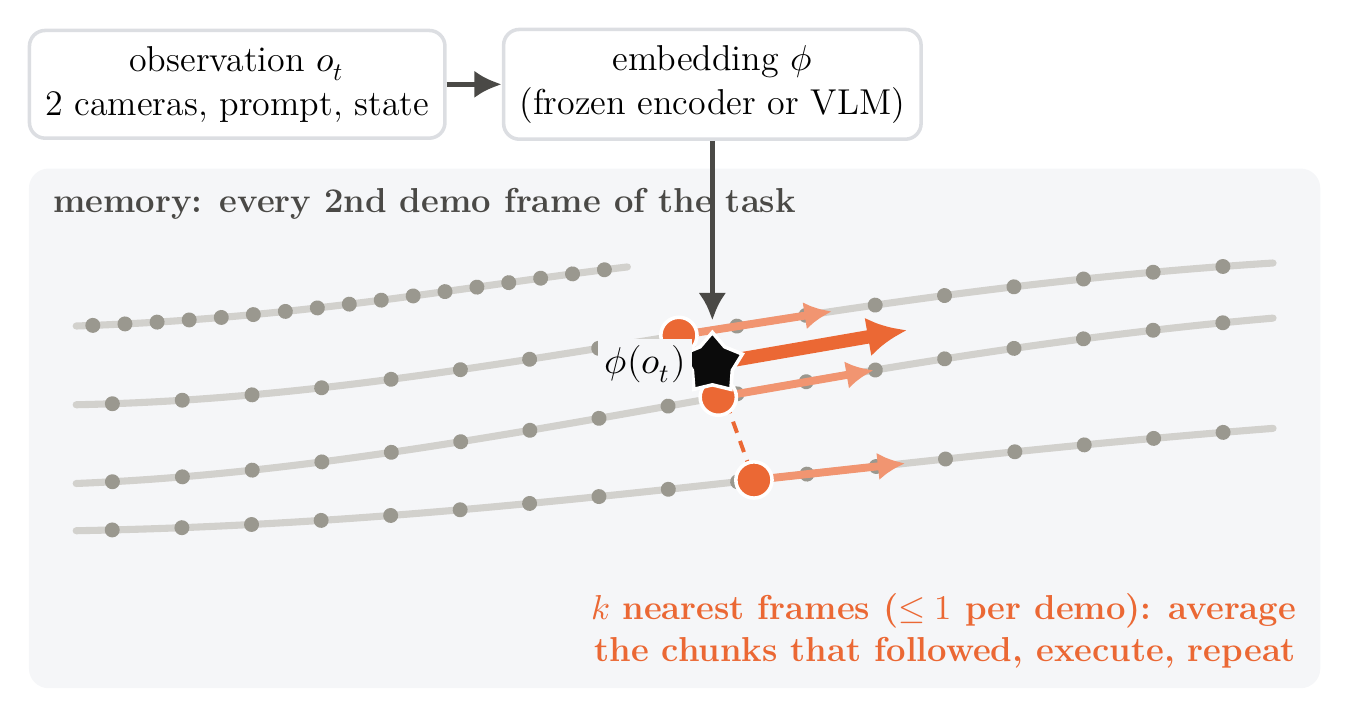
\begin{tikzpicture}[x=1cm,y=1cm,font=\fontsize{13}{16}\selectfont,
    demo/.style={line width=0.9mm, draw=human!45, line cap=round},
    dots/.style={postaction={decorate}, decoration={markings,
        mark=between positions 0.03 and 0.97 step 0.058 with {\fill[human] (0,0) circle (0.95mm);}}},
    nb/.style={circle, fill=knn, draw=white, line width=0.45mm, minimum size=4.6mm, inner sep=0},
    box/.style={rounded corners=2mm, draw=hair, line width=0.45mm, fill=panel, align=center, inner sep=2mm}]
  \fill[tint, rounded corners=2.5mm] (0,0) rectangle (16.4,6.6);
  \draw[demo, dots] (0.6,2.6) .. controls (5.5,2.8) and (10,4.2) .. (15.8,4.7) coordinate[pos=0.56](a) coordinate[pos=0.69](a2);
  \draw[demo, dots] (0.6,3.6) .. controls (5.5,3.7) and (9.5,5.0) .. (15.8,5.4) coordinate[pos=0.54](b) coordinate[pos=0.67](b2);
  \draw[demo, dots] (0.6,2.0) .. controls (6,2.1) and (10,2.85) .. (15.8,3.3) coordinate[pos=0.58](c) coordinate[pos=0.71](c2);
  \draw[demo, dots] (0.6,4.6) .. controls (3.5,4.7) and (5.5,5.1) .. (7.6,5.35);
  \coordinate (q) at ($(a)!0.45!(b)+(0.15,0.07)$);
  % query path: observation -> phi -> point in the memory
  \node[box] (phi) at ($(q)+(0,3.55)$) {embedding $\phi$\\(frozen encoder or VLM)};
  \node[box, left=7mm of phi] (obs) {observation $o_t$\\2 cameras, prompt, state};
  \draw[-{Latex[length=3.5mm,width=3.5mm]}, line width=0.7mm, ink2] (obs) -- (phi);
  \draw[-{Latex[length=3.5mm,width=3.5mm]}, line width=0.7mm, ink2] (phi.south) -- ($(q)+(0,0.55)$);
  \foreach \n in {a,b,c} \draw[knn, line width=0.5mm, dash pattern=on 1.5mm off 1.1mm] (q) -- (\n);
  \foreach \n/\m in {a/a2,b/b2,c/c2} {\draw[-{Latex[length=3.5mm,width=3.5mm]}, line width=1mm, knn!70] (\n) -- (\m);
                                      \node[nb] at (\n) {};}
  \draw[-{Latex[length=5mm,width=5mm]}, line width=1.7mm, knn] (q) -- ($(q)+1.25*($(a2)-(a)$)$);
  \node[star, star points=5, fill=ink, draw=white, line width=0.45mm, minimum size=8mm, inner sep=0] at (q) {};
  \node[left=2.5mm of q, font=\fontsize{13.5}{15}\selectfont\bfseries, fill=tint, inner sep=0.8mm] {$\phi(o_t)$};
  \node[anchor=north west, font=\fontsize{12.5}{15}\selectfont\bfseries, text=ink2, inner sep=1mm] at (0.2,6.45)
    {memory: every 2nd demo frame of the task};
  \node[anchor=south east, font=\fontsize{12.5}{15}\selectfont\bfseries, text=knn, align=right, inner sep=1mm]
    at (16.2,0.15) {$k$ nearest frames ($\le 1$ per demo): average\\the chunks that followed, execute, repeat};
\end{tikzpicture}

\begin{itemize}
  \item \textbf{Memory}: every 2nd frame of the 1{,}693 demonstrations (137k keys) with the chunk that followed.
        ``Training'' is embedding them: minutes, no gradient step.
  \item \textbf{Key} $\phi$: ResNet-18 layer 3 on a 4$\times$4 grid per camera; for a VLA, one layer's hidden states
        over each camera's image tokens, standardised and pooled to a 2$\times$2 grid.
  \item \textbf{Distance}: image distance per camera, plus state, prompt (CLIP), time-in-episode and history
        terms, each scaled by the task's median.
  \item \textbf{Retrieve}: the $k$ nearest frames, at most one per demonstration, softmax-weighted.
  \item \textbf{Mode seeking}: neighbours whose chunks disagree with the dominant one are down-weighted instead of
        averaged into an action no demonstrator took. Every action stays inside its neighbours' convex hull.
  \item \textbf{Temporal ensembling}: overlapping chunk predictions, exponentially weighted (as in ACT).
  \item \textbf{Retry} (option, off): rewind and retrieve again when the scene looks unseen or the arm is stuck;
        no gain on LIBERO-Long (\RetryBase\% $\to$ \RetryMin--\RetryMax\%).
\end{itemize}

\block{Tuning}
Optuna searched all of the above: \OptunaAll\ trials of 400 episodes on initial states 40--49 and 0--19 (LIBERO has no
held-out split, so the official evaluation includes them, as for every LIBERO result); $k$ and \emph{at most one per
demonstration} explain \OptunaK\% and \OptunaOne\% of the variance. Without the prompt success falls to \AblNoLang\%,
with raw pixels as the key to \AblPixels\%, with 10\% of the demos to \DemosTen\%: \hl{the representation, the prompt
and the data do the work.}

\block{What a key encodes}
\fig{embedding_pairs.pdf}
t-SNE of each key on the same \MapN\ demo frames; below: same-task neighbours in LIBERO-Goal (one scene, ten
instructions) and the median progress gap to the nearest frame of another demo. \textbf{Fine-tuning makes VLM keys
track the task's phase} (\MapPhaseDown\ of \MapPhaseN; Evo-1 \MapPhaseEvoBefore\,$\to$\,\MapPhaseEvoAfter); $\pi_0$'s
keeps the task but loses the phase (\MapPhasePiZeroAfter): its lookup falls to \KnnPiZeroLt\%.
}

% ============================================ MIDDLE ========================================================
\posterbox{name=middle, column=2, between=header and footer}{%
\sectionhead{2}{How hard is the task?}

\textbf{LIBERO}: 4 suites $\times$ 10 tasks, $\sim$42 demonstrations per task; every policy on the official
protocol, 50 episodes per task (2{,}000). \textbf{LIBERO-plus}: the same 40 tasks under seven perturbations; a fixed sample of \PlusN\ of its 10{,}030 variants (\PlusPerCat\ per perturbation), the same for every policy, never trained on. \textbf{VLAs}: nine public LeRobot Hub LIBERO fine-tunes.

\block{Success on LIBERO and LIBERO-plus}
\par\vspace{1mm}{\fontsize{12}{15.5}\selectfont\setlength{\tabcolsep}{1.6pt}\begin{tabularx}{\linewidth}{@{}l*{5}{>{\raggedleft\arraybackslash}X}@{\hspace{3mm}}*{5}{>{\raggedleft\arraybackslash}X}@{\hspace{3mm}}>{\raggedleft\arraybackslash}X@{}}
\toprule
 & \multicolumn{5}{c}{LIBERO} & \multicolumn{5}{c}{LIBERO-plus} & \\
\cmidrule(lr){2-6}\cmidrule(lr){7-11}
 & avg & Spat & Obj & Goal & Long & avg & Spat & Obj & Goal & Long & drop \\
\midrule
$\pi_{0.5}$ & \textbf{97.7} & 97 & 100 & \textbf{98} & \textbf{96} & \textbf{85.5} & \textbf{90} & 84 & 83 & \textbf{85} & −12.2 \\
MolmoAct2 & 97.5 & \textbf{97} & 99 & 98 & 96 & 82.6 & 90 & 82 & 76 & 83 & −14.9 \\
\rowcolor{tint}\knnword{}, full method & 91.7 & 88 & 100 & 98 & 81 & 82.4 & 79 & \textbf{86} & \textbf{87} & 78 & \textbf{−9.3} \\
\rowcolor{tint}\knnword{}, + learnt key & 93.0 & 91 & 100 & 97 & 85 & 81.7 & 88 & 84 & 81 & 74 & −11.3 \\
GR00T N1.7 & 94.8 & 96 & 98 & 95 & 91 & 80.2 & 90 & 74 & 79 & 78 & −14.6 \\
\rowcolor{tint}\knnword{}, plain & 88.7 & 90 & 95 & 95 & 74 & 75.5 & 77 & 82 & 79 & 64 & −13.2 \\
VLA-JEPA & 97.2 & 95 & \textbf{100} & 97 & 96 & 74.0 & 81 & 70 & 77 & 68 & −23.1 \\
Evo-1 & 95.4 & 92 & 99 & 97 & 94 & 71.4 & 74 & 73 & 70 & 69 & −24.0 \\
X-VLA & 94.5 & 95 & 99 & 93 & 92 & 64.5 & 71 & 65 & 65 & 57 & −30.0 \\
$\pi_0$ & 71.9 & 70 & 86 & 86 & 45 & 42.9 & 54 & 42 & 47 & 29 & −29.0 \\
SmolVLA & 82.2 & 79 & 92 & 88 & 70 & 27.9 & 30 & 50 & 11 & 20 & −54.3 \\
$\pi_0$-FAST & 90.5 & 90 & 94 & 91 & 87 & 25.7 & 39 & 34 & 16 & 13 & −64.8 \\
\bottomrule
\end{tabularx}
\par}\vspace{1.5mm}
Ordered by LIBERO-plus success; bold: best per column. The kNN rows are \textbf{training-free}, except the learnt
key (one linear map per grid cell); \emph{plain}: ImageNet ResNet-18 key, none of the extras.
\textbf{A training-free lookup is competitive}: \KnnAvg\% on LIBERO, rank \KnnRankLibero\ of \RankN.
\textbf{Under perturbation it ranks \KnnRankPlus\ and degrades least}: \KnnDrop\ points, against \MinVlaDrop\ for
the most robust VLA and up to \MaxVlaDrop; it is the best of all on \KnnBestPlusSuites\ suites.

\block{The same tasks are hard for everyone}
\fig{task_map.pdf}
\textbf{VLAs fail where the lookup fails}: when a VLA fails a LIBERO episode, the lookup fails the same episode in
\FailMin--\FailMax\% of cases, against \FailBase\% overall (\LiftMin--\LiftMax$\times$ chance), and per-task success
correlates with the lookup's (median $r$\,=\,\TaskCorrMedian). The extra episodes the best VLAs solve are a few
long-horizon ones. Under perturbation the collapsing VLAs fail almost everywhere.

\block{What breaks under perturbation}
\fig{libero_plus.pdf}
\textbf{Weak VLAs key on the wording}: reworded instructions over the original scenes drop SmolVLA, $\pi_0$-FAST
and $\pi_0$ to \PlusSmolLanguage, \PlusFastLanguage\ and \PlusPiZeroLanguage\% (original wording: \PlusSmolCtrl,
\PlusFastCtrl, \PlusPiZeroCtrl\%): they memorised 40 instructions. X-VLA fails under a camera shift
(\PlusXvlaCamera\%). The lookup suffers most from new robot initial states and object layouts.
}

\posterbox[colback=titlebg, colframe=titlebg, colupper=white, left=8mm, right=8mm, top=7mm, bottom=7mm,
           before upper={\setlength{\parskip}{0.5em}\raggedright}]{name=conclusions, column=3, above=footer}{%
  {\display\bfseries\fontsize{22}{26}\selectfont Conclusions\par}
  {\fontsize{15}{19}\selectfont\color{white!85!titlebg}We do not propose a lookup for robot control. It is a
   \textbf{simple, training-free test} for three questions:\par}
  \begin{itemize}\fontsize{14.5}{18.5}\selectfont
    \item \textbf{How hard is your task?} If a lookup over the demos solves it (LIBERO: \KnnAvg\%), success there
          measures memorisation: VLAs fail on the same tasks, and lose up to \MaxVlaDrop\ points off the demos.
    \item \textbf{How good is your backbone, and what did fine-tuning do to it?} A lookup on its VLM before and
          after fine-tuning (or LAC, without rollouts). Fine-tuning mostly makes it a more robust key (+\FtUpMin\ to
          +\FtUpMax\ under perturbation), or breaks it ($\pi_0$).
    \item \textbf{How good is your action head?} Its margin over that lookup: \BeatenClean\ of \KeyN\ fall below it.
  \end{itemize}
  {\fontsize{14}{18}\selectfont\color{white!72!titlebg}Report a kNN baseline with every result on a
   dense-demonstration benchmark.\par}
}

% ============================================ RIGHT =========================================================
\posterbox{name=right, column=3, between=header and conclusions}{%
\sectionhead{3}{Inside the VLAs}

\block{VLAs act like a lookup}
Clean LIBERO rollouts: a lookup over the demos (ResNet-18 key, $k$\,=\,8) predicting each VLA's chunk at the same
state, and the chunk's distance to the nearest training chunk.
\fig{vla_lookup.pdf}
\textbf{A lookup predicts a VLA's actions} as well as a human's, or better (R$^2$ \LookupPi\ for $\pi_{0.5}$,
\LookupHuman\ for human demos), and \textbf{its actions are not new}: closer to a training chunk than a new human demo
is. On LIBERO-plus the robust VLAs stay lookup-like (R$^2$ \HeadPlusPi\ for $\pi_{0.5}$), the collapsing ones do not
(\HeadPlusFast\ for $\pi_0$-FAST). {\color{ink2}$^\dagger$Spatial suite; X-VLA (absolute poses) left out.}

\block{Backbone and action expert, before and after fine-tuning}
A lookup on a VLA's own VLM scores its \textbf{backbone}; the VLA's excess over it is its \textbf{action
expert}'s (VLM before / after LIBERO fine-tuning, \%):
\par\vspace{1mm}{\fontsize{13.5}{17.5}\selectfont\setlength{\tabcolsep}{3pt}\begin{tabularx}{\linewidth}{@{}l*{6}{>{\raggedleft\arraybackslash}X}@{}}
\toprule
 & \multicolumn{3}{c}{LIBERO} & \multicolumn{3}{c}{LIBERO-plus} \\
\cmidrule(lr){2-4}\cmidrule(lr){5-7}
 & \knnword{} before & \knnword{} after & VLA & \knnword{} before & \knnword{} after & VLA \\
\midrule
$\pi_{0.5}$ & 85.4 & 81.8 & \textcolor{learned}{97.7} & 60.5 & 65.7 & \textcolor{learned}{85.5} \\
MolmoAct2 & 78.6 & 91.3 & \textcolor{learned}{97.5} & 52.6 & 81.0 & \textcolor{learned}{82.6} \\
GR00T N1.7* & 87.5 & 87.5 & \textcolor{learned}{94.8} & 66.4 & 66.4 & \textcolor{learned}{80.2} \\
VLA-JEPA & 84.0 & 83.0 & \textcolor{learned}{97.2} & 49.3 & 65.7 & \textcolor{learned}{74.0} \\
Evo-1 & 62.1 & 87.1 & \textcolor{learned}{95.4} & 35.5 & \textcolor{knn}{\textbf{72.6}} & \textcolor{learned}{71.4} \\
X-VLA & 83.3 & 88.5 & \textcolor{learned}{94.5} & 62.4 & \textcolor{knn}{\textbf{78.1}} & \textcolor{learned}{64.5} \\
$\pi_0$ & 86.9 & 17.9 & \textcolor{learned}{71.9} & 56.7 & 2.4 & \textcolor{learned}{42.9} \\
SmolVLA & 76.3 & \textcolor{knn}{\textbf{86.5}} & \textcolor{learned}{82.2} & 45.0 & \textcolor{knn}{\textbf{69.3}} & \textcolor{learned}{27.9} \\
$\pi_0$-FAST & 86.6 & \textcolor{knn}{\textbf{95.0}} & \textcolor{learned}{90.5} & 58.3 & \textcolor{knn}{\textbf{74.0}} & \textcolor{learned}{25.7} \\
\bottomrule
\end{tabularx}
\par}\vspace{1.5mm}
\textbf{Fine-tuning makes a VLM a more robust key} (+\FtUpMin\ to +\FtUpMax\ on LIBERO-plus, \FtUp\ of \FtN\ VLAs;
clean: \FtCleanUp); $\pi_0$'s breaks it (\KnnPiZeroBaseLt\,$\to$\,\KnnPiZeroLt\%). \textbf{Some action experts
subtract} (orange): \BeatenClean\ of \KeyN\ VLAs fall below a lookup on their own VLM, \BeatenPlus\ of \KeyNPlus\ under
perturbation (up to \SubtractMax\ points). $^{*}$GR00T froze its VLM.

\block{Scoring a backbone without rollouts}
\textbf{Local action consistency}: LAC@8\,=\,1\,$-$ action distance to a key's 8 nearest frames of other
demos\,/\,to a random frame of the task (held-out queries).
\fig{neighbors.pdf}
\textbf{LAC tracks backbones} ($r$\,=\,\NmFairR, $\rho$\,=\,\NmFairRho; \NmFairN\ keys) and flags a broken one ($\pi_0$
fine-tuned: \NmPiZeroLibero). \textbf{As a loss it improves a key}: a linear map per ResNet grid cell lifts the lookup
\KnnPlainResnet\,$\to$\,\hl{\KnnLearnt\%}.
}
\end{tcbposter}
\end{document}
